
\begin{figure}[p]

    \noindent\makebox[\textwidth]{
        \centering
        %\includegraphics[width=0.8\textwidth]{../../sympy/catalan/coloured.pdf}

        % using *angle* property to rotate it is difficult to properly align it
        % in order to have a "real" matrix representation.
        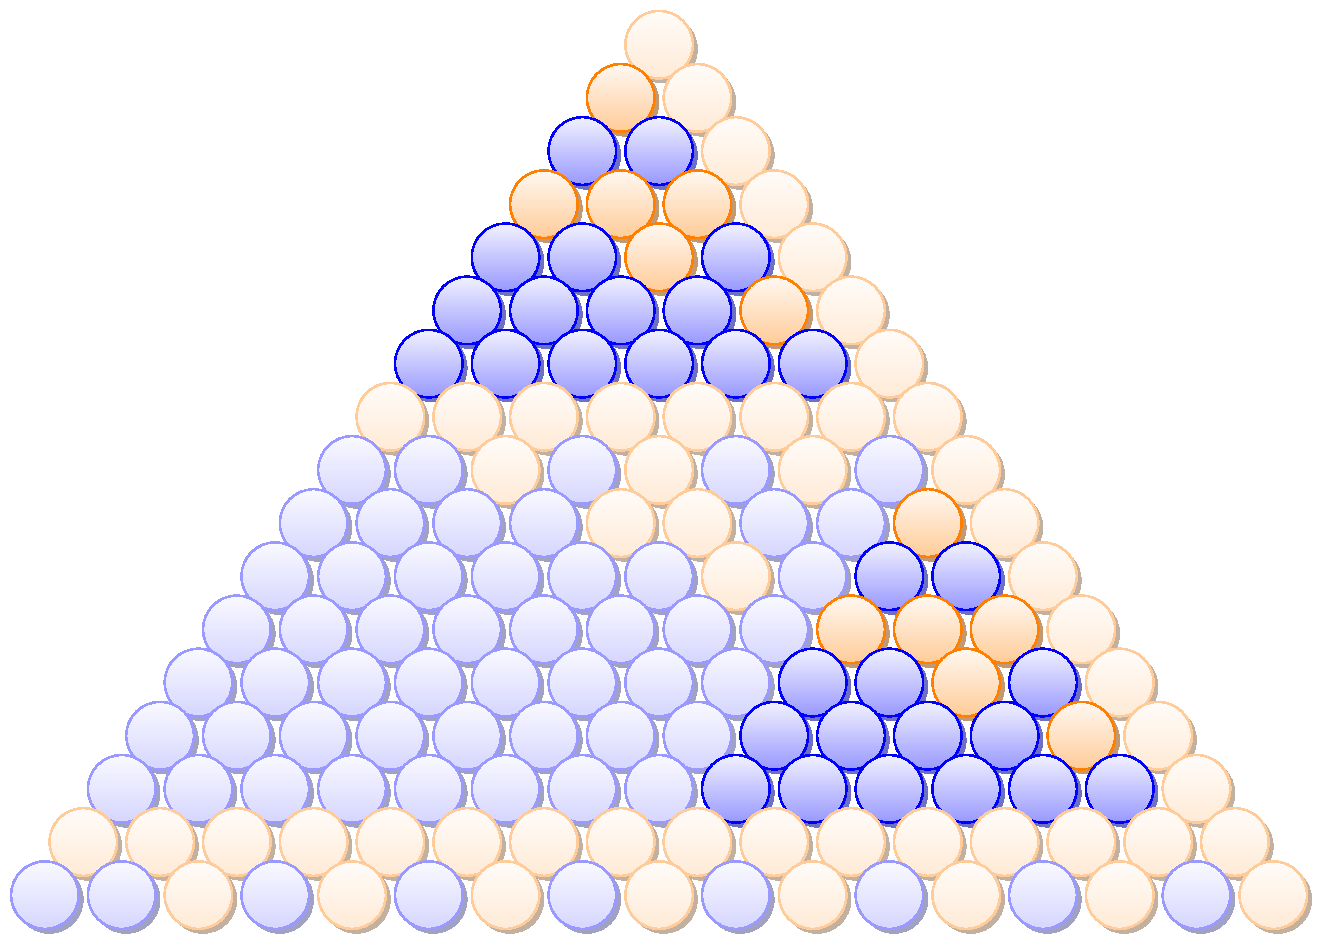
\includegraphics[width=6cm, height=6cm, keepaspectratio=true]{../RART2015/catalan-tikz/principal-cluster/principal-cluster.pdf}
    }

    % this 'particular' line is necessary to use `displaymath' environment
    % into the caption environment, togheter with the inclusion of 
    % `caption' package. See here for more explanation:
    % http://stackoverflow.com/questions/2716227/adding-an-equation-or-formula-to-a-figure-caption-in-latex
    \captionsetup{singlelinecheck=off}
    \caption[$\mathcal{C}_{\equiv_{2}}^{(4)}$ 
    contains a copy of $\mathcal{C}_{\equiv_{2}}^{(3)}$]{$\hat{d}_{s,2^{3}-1}$ for $s\in S_{2^{3}-1}$,
    $d_{s,2^{3}-1+e} \equiv_{2} d_{s-2^{3},e-1}$ with $e\in\lbrace1,\ldots,s-2^{3}\rbrace$ }

    \label{fig:catalan-principal-cluster}

\end{figure}
